\section{Holography introduction}

Antenna holography is procedure with the goal of measuring the antenna positioning imperfections to later correct them. 

The ideal cassegrain antenna is composed by a big main dish with a paraboloidal form and a subreflector with an hyperboloid geometry.
While the subreflector can be build with just a single metallic piece, the main parabolic dish is normally build placing several panels that composed the desired geometry. In figure \ref{fig:apex_diagram} you can see the APEX diagram as example.


\begin{figure}[h]
    \centering
    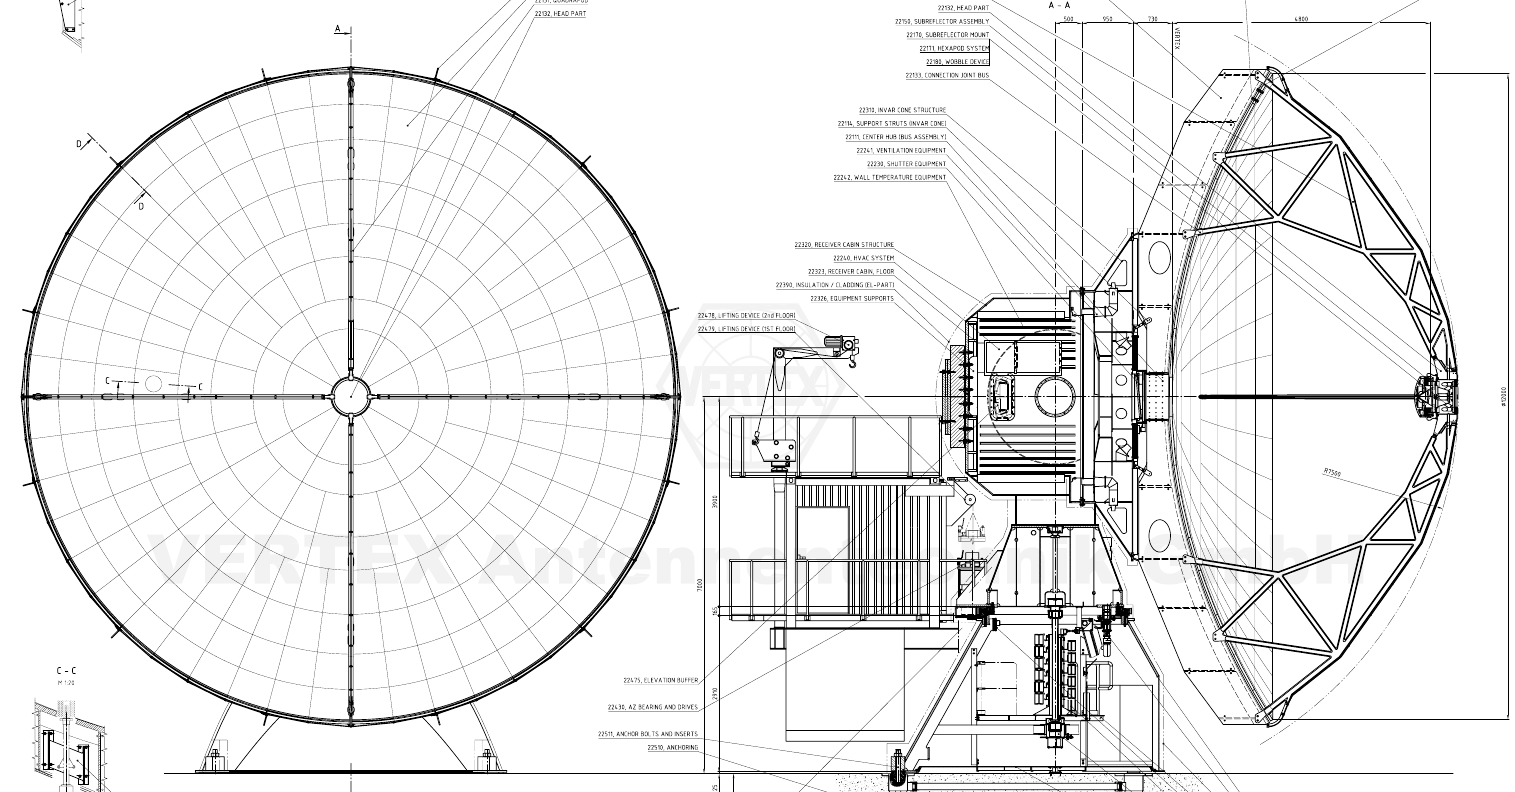
\includegraphics[width=0.8\textwidth]{images/apex_diagram.png}
    \caption{APEX telescope diagram.}
    \label{fig:apex_diagram}
\end{figure}


The accuracy of the panel positioning affects directly the efficiency of the overall antenna, you can think of it as that as worst the surface of the antenna you are not collecting all the power in the foci. The rule of thumbs is that the main dish should have an error in the positioning of the panels of around $\lambda/16$ where $\lambda$ is the wavelength beign observed, for our 850GHz receiver this limits the error to be 22$\mu$m RMS as max.


Each panel has 5 micrometer adjustment screws that can be used to re-position it, in figure \ref{fig:apex_panel} there is a diagram of one of the APEX panels. 
The 5 degrees of freedom in a panel can correct piston (if the panel has a global positive/negative offset), tilts and first order mechanical torsions.
These type of deformations can be modeled as equation \ref{eq:panel_deformation} where (x,y) are the local coordinates from each panel shown in the figure \ref{fig:apex_panel}(more on that later..).

\begin{figure}[t]
    \centering
    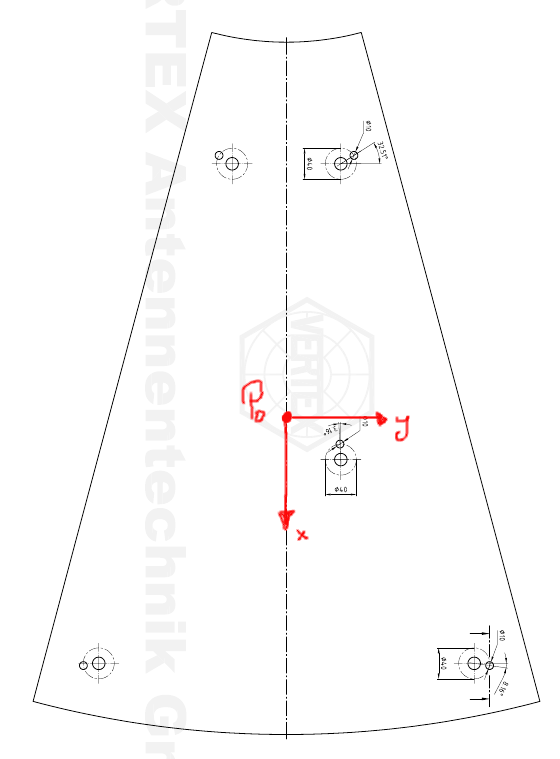
\includegraphics[width=0.5\textwidth]{images/apex_panel_diag_coord.png}
    \caption{APEX panel example.}
    \label{fig:apex_panel}
\end{figure}


\begin{equation}
    f_{\text{Panel}_i}(x,y) = a_i+b_i\cdot x + c_i \cdot y + d_i\cdot (x^2+y^3) + e_i \cdot (x^2-y^2)
    \label{eq:panel_deformation}
\end{equation}


To measure the surface of the antenna we make a map of its beam pattern. The beam pattern of one antenna can be roughly defined as the way that one antenna emits/receive power for different positions. So for example the desired antenna for radioastronomy is one that only sense a small region in the sky with a huge gain, therefore you can direct it to one astronomical source and be sure that you are just looking that.

In the figure \ref{fig:apex_beam} there is an example of the beam pattern measured at APEX at 92GHz, where you can see that most of the power is beign captured/emited in a small angular region near the $0^{\circ}$. To measure the beam pattern of the antenna you place a transmitter at some given distance and then start to move the antenna around it to get the received power in different positions.

\begin{figure}[h]
    \centering
    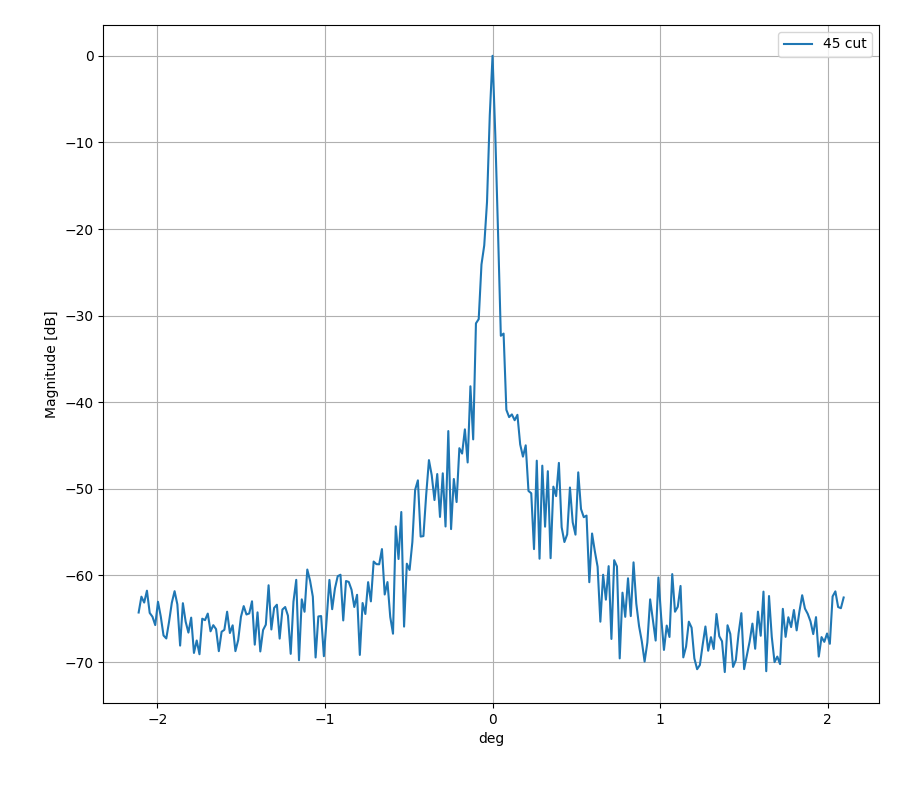
\includegraphics[width=0.5\textwidth]{images/Measured_dB_cut45.png}
    \caption{APEX beam pattern cut.}
    \label{fig:apex_beam}
\end{figure}

The beam pattern of one antenna is related to the induced currents in the main dish, and therefore to the deviations of the position of the panels. As always, the actual expressions are awfull, but with some approximations you can find that the relation between the beam pattern and the currents is just a 2D Fourier transform + some corrections that you need to do over the data.

To truly invert a Fourier transform you need to measure amplitude and phase, then an holography system usually measure the complex beam pattern and got maps like the following at figure \ref{fig:apex_holo_map}. After the processing we got the surface error maps shown at the left in figure \ref{fig:apex_errors}. 

With the final surface error we iterate over the panels area doing a fitting with the deformation function at equation \ref{eq:panel_deformation} \footnote{Note that here there is a subtle trick: since in the standard method we project the errors to a plane, then in this case (x,y) are not curved and can be taken as the usual cartesian coordinates}. and finally we can compute the turns that we need to give to the screw adjuster of each panel.


\begin{figure}[t]
    \centering
    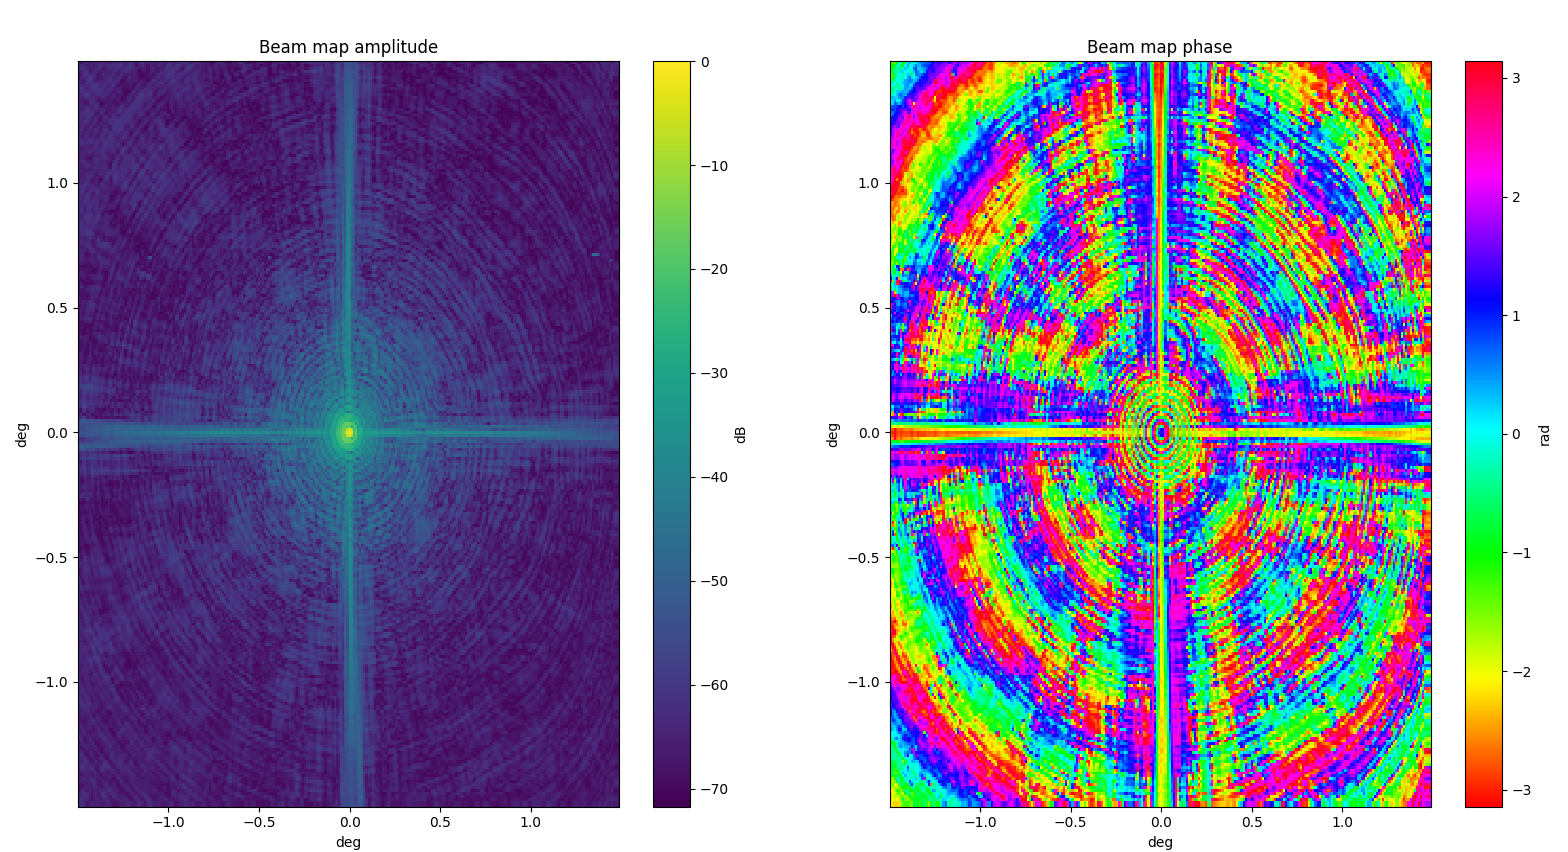
\includegraphics[width=0.7\textwidth, height=0.35\textwidth]{images/holo_beam_map_ex.png}
    \caption{APEX holography map.}
    \label{fig:apex_holo_map}
\end{figure}


\begin{figure}[h]
    \centering
    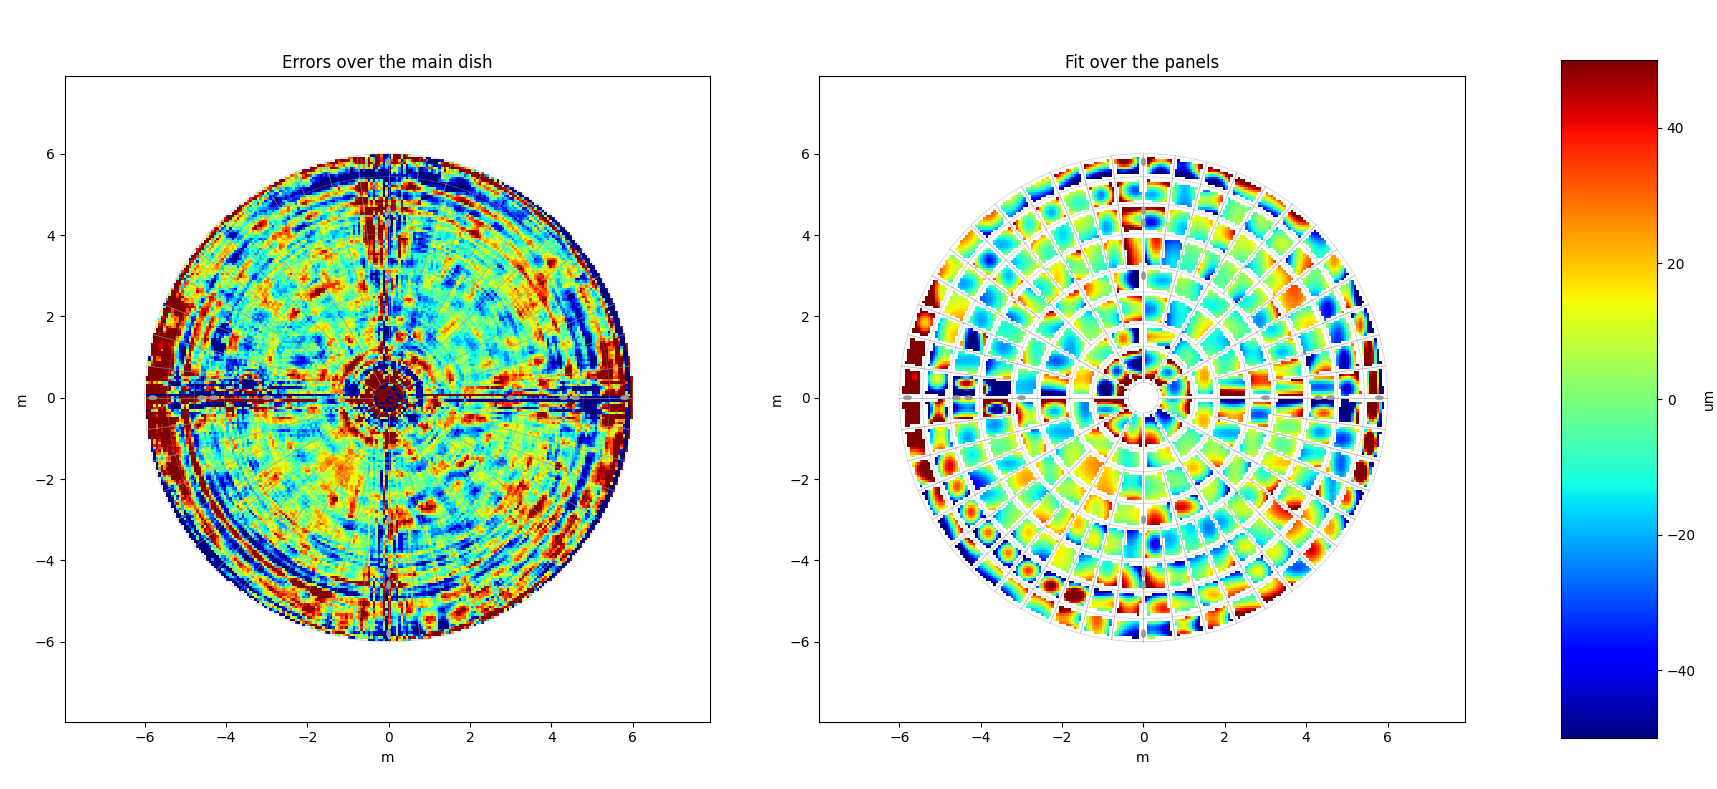
\includegraphics[width=0.75\textwidth, height=0.4\textwidth]{images/example_of_final_error.png}
    \caption{Derived surface error and the fit over the panels.}
    \label{fig:apex_errors}
\end{figure}













